% --------------------------------------------------------------
% This is all preamble stuff that you don't have to worry about.
% Head down to where it says "Start here"
% --------------------------------------------------------------

\documentclass[12pt]{article}

\usepackage[margin=1in]{geometry}
\usepackage{amsmath,amsthm,amssymb}
\usepackage{graphicx} %This allows to include eps figures

% This is to include code
\usepackage{listings}
\usepackage{xcolor}
\usepackage{caption}
\usepackage{subcaption}
\definecolor{dkgreen}{rgb}{0,0.6,0}
\definecolor{gray}{rgb}{0.5,0.5,0.5}
\definecolor{mauve}{rgb}{0.58,0,0.82}
\lstdefinestyle{Python}{
    language        = Python,
    basicstyle      = \ttfamily,
    keywordstyle    = \color{blue},
    keywordstyle    = [2] \color{teal}, % just to check that it works
    stringstyle     = \color{green},
    commentstyle    = \color{red}\ttfamily
}

\newcommand{\N}{\mathbb{N}}
\newcommand{\Z}{\mathbb{Z}}

\newenvironment{theorem}[2][Theorem]{\begin{trivlist}
\item[\hskip \labelsep {\bfseries #1}\hskip \labelsep {\bfseries #2.}]}{\end{trivlist}}
\newenvironment{lemma}[2][Lemma]{\begin{trivlist}
\item[\hskip \labelsep {\bfseries #1}\hskip \labelsep {\bfseries #2.}]}{\end{trivlist}}
\newenvironment{exercise}[2][Exercise]{\begin{trivlist}
\item[\hskip \labelsep {\bfseries #1}\hskip \labelsep {\bfseries #2.}]}{\end{trivlist}}
\newenvironment{reflection}[2][Reflection]{\begin{trivlist}
\item[\hskip \labelsep {\bfseries #1}\hskip \labelsep {\bfseries #2.}]}{\end{trivlist}}
\newenvironment{proposition}[2][Proposition]{\begin{trivlist}
\item[\hskip \labelsep {\bfseries #1}\hskip \labelsep {\bfseries #2.}]}{\end{trivlist}}
\newenvironment{corollary}[2][Corollary]{\begin{trivlist}
\item[\hskip \labelsep {\bfseries #1}\hskip \labelsep {\bfseries #2.}]}{\end{trivlist}}

\begin{document}

% --------------------------------------------------------------
%                         Start here
% --------------------------------------------------------------

%\renewcommand{\qedsymbol}{\filledbox}

\title{Homework 3}%replace X with the appropriate number
\author{Thomas Buchegger\\ %replace with your name
Introduction to Signal and Image Processing}
\maketitle

\setcounter{tocdepth}3 % Set the depth of the table of contents to show sections and subsections only
\tableofcontents

\pagebreak
\section{Introduction}
This assignment is about the RANSAC algorithm and texture synthesis with SSD.
\newline

RANSAC (random sample consensus) is a rather simple algorithm designed to cope with a large proprtion of outliners in input data.
It is a resampling technique which generates different solutions by using the minimum number of data points required to estimate 
the underlying model parameters. Unlike other estimation techniques which use as much data as possible, RANSAC only uses the smallest 
possible set and proceeds to enlarge this set with consistent data points.
\newline
\newline
Texture Synthesis is used to fill an empty section of an image with a reconstruction based on a SSD (Sum Squared Difference) approach. 
This means, the algorithm selects pixel on be boundary of the to be filled space and then calculates the SSD. So a pixel from the sample set 
is used to substitute a pixel from the empty space.

\pagebreak

\section{Ransac}
\subsection{Introduction}
 As mentioned, RANSAC is a method for iteratively estimate the parameters of a mathematical model from a set of data with outliners.
 The goal of this assignment was to detect lines on an image and plot them. The algorithm works as follows:

 \begin{enumerate}
     \item Select randomly minimum number of points to determine the model parameters
     \item Solve for the parameter of the model
     \item Determine how many points from the set of all points fit with a predefinded tolerance
     \item If fraction of number of inliners over the total number points in the set exceed a predefined threshold, re-estimate model parameters using all identified inliners and terminate
     \item Else, repeate steps 1 to 4 (N iterations)
 \end{enumerate}
 
 The number of iterations should be chosen high to ensure that at least one set of random samples does not include any outliners.

\subsection{Exercises}
\subsubsection{edge\_map}
To get an edge map out of the picture, I used a canny edge algorithm with sigma 1.5. The results where satisfying and calculation time was within
acceptance. 
\subsubsection{fit\_line}
A linear function has the two parameters m and c. The task was to get the slope of the fitted line m and the y-intersect of the fitted line.
This could be achieved with subtracting the coordinate points. To avoid division by zero, we add some noise $\epsilon$.
\subsubsection{point\_to\_line\_dist}
As for the distribution, I used the following formula: $dist = \frac{|m \cdot x_{0} - y_{0} + c|}{\sqrt{m^2+1}}$

\pagebreak
\subsection{Results}
The following pictures are the results with the ransac algorithm. The used parameters are:
\begin{itemize}
    \item Iterations = 500
    \item Threshold = 2
    \item n samples = 2
    \end{itemize}

\begin{figure}[!htb]
  \centering
  \begin{subfigure}{.5\textwidth}
    \centering
    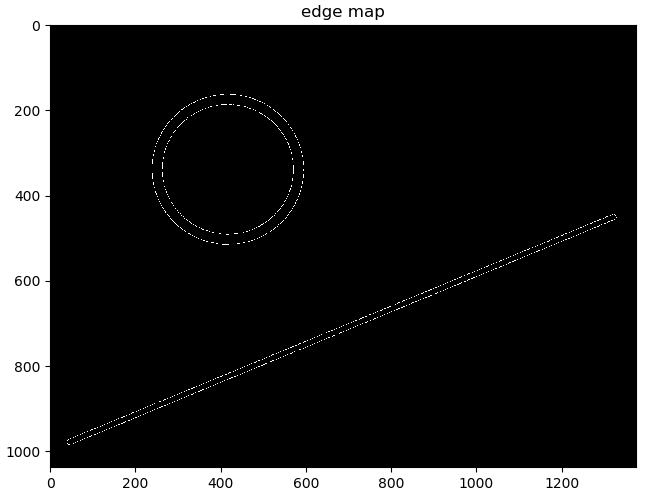
\includegraphics[width=0.95\linewidth]{pics/syntheticEdgeMap}
    \caption{edge map}
  \end{subfigure}%
  \begin{subfigure}{.5\textwidth}
    \centering
    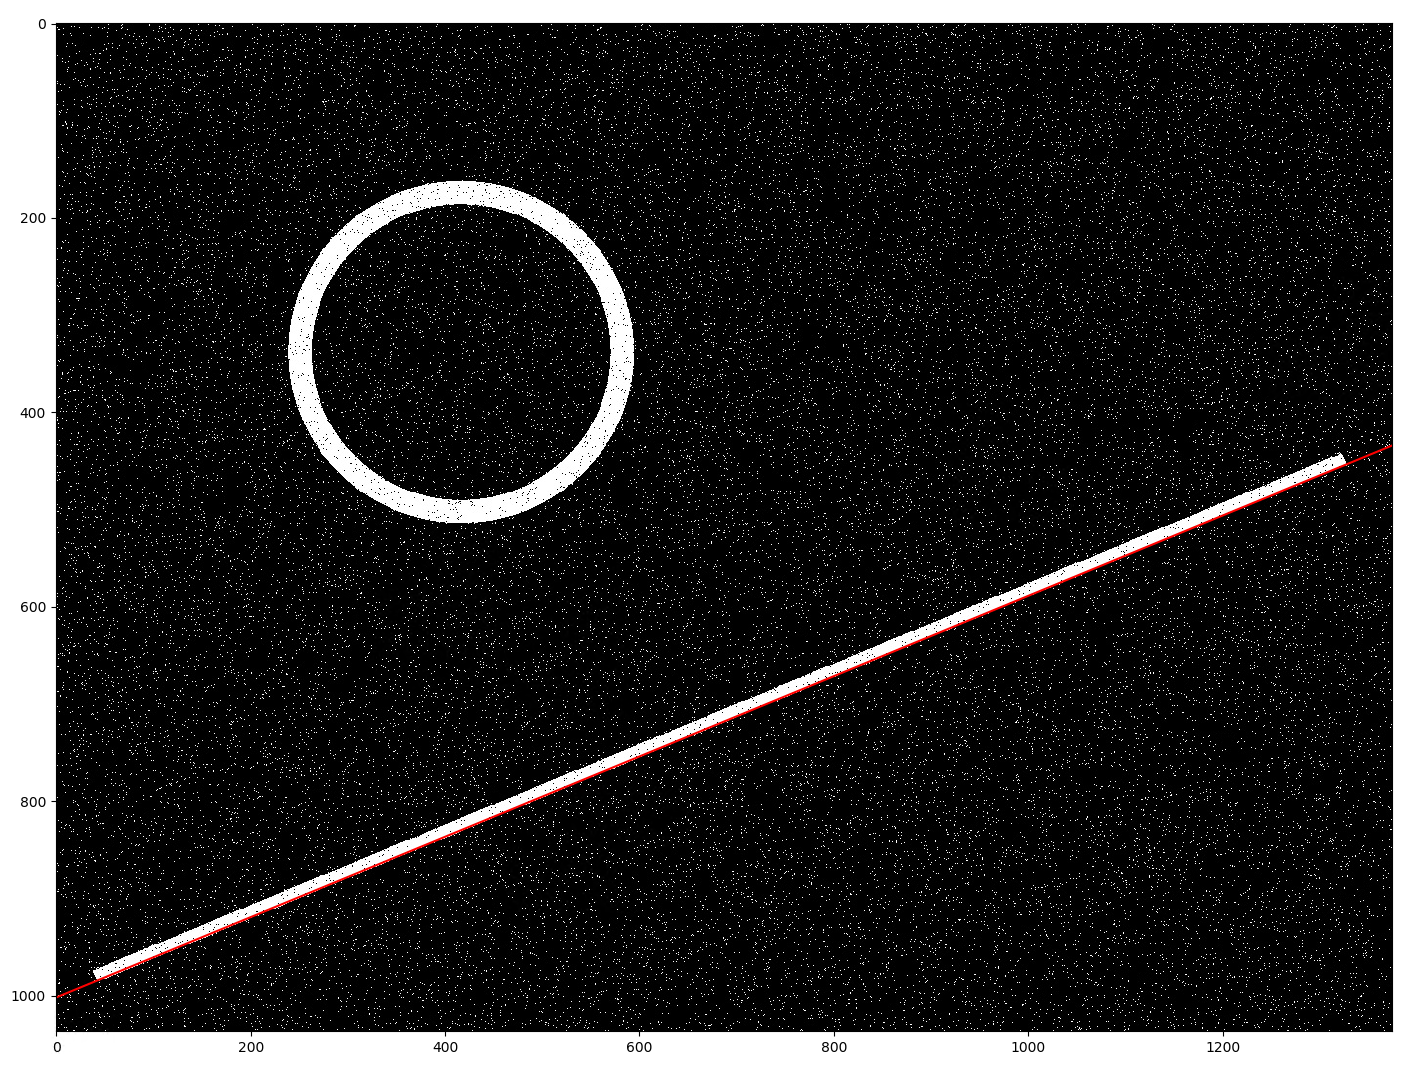
\includegraphics[width=0.95\linewidth]{pics/synthetic}
    \caption{result}
   \end{subfigure}
  \caption{Calculations of synthetic.jpg}
\end{figure}

\begin{figure}[!htb]
  \centering
  \begin{subfigure}{.5\textwidth}
    \centering
    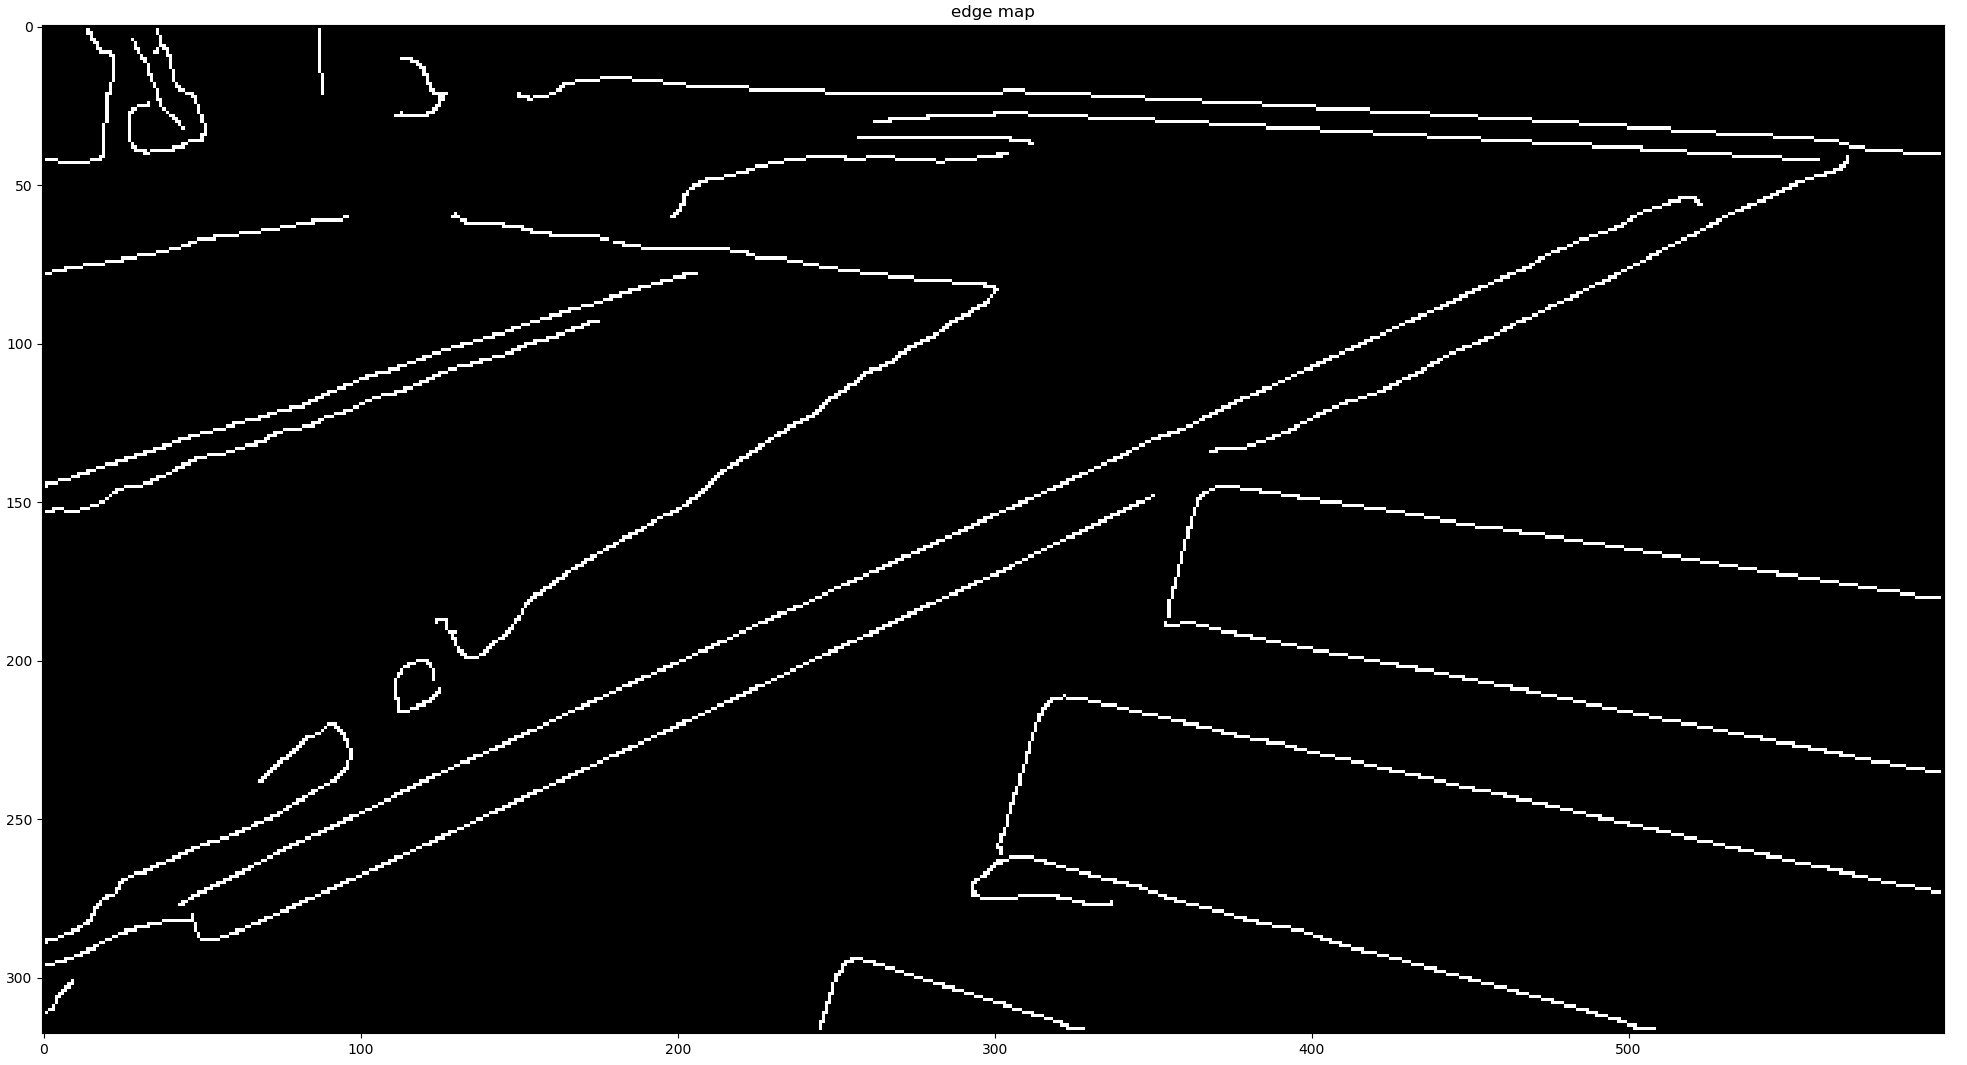
\includegraphics[width=0.95\linewidth]{pics/poolEdgeMap}
    \caption{edge map}
  \end{subfigure}%
  \begin{subfigure}{.5\textwidth}
    \centering
    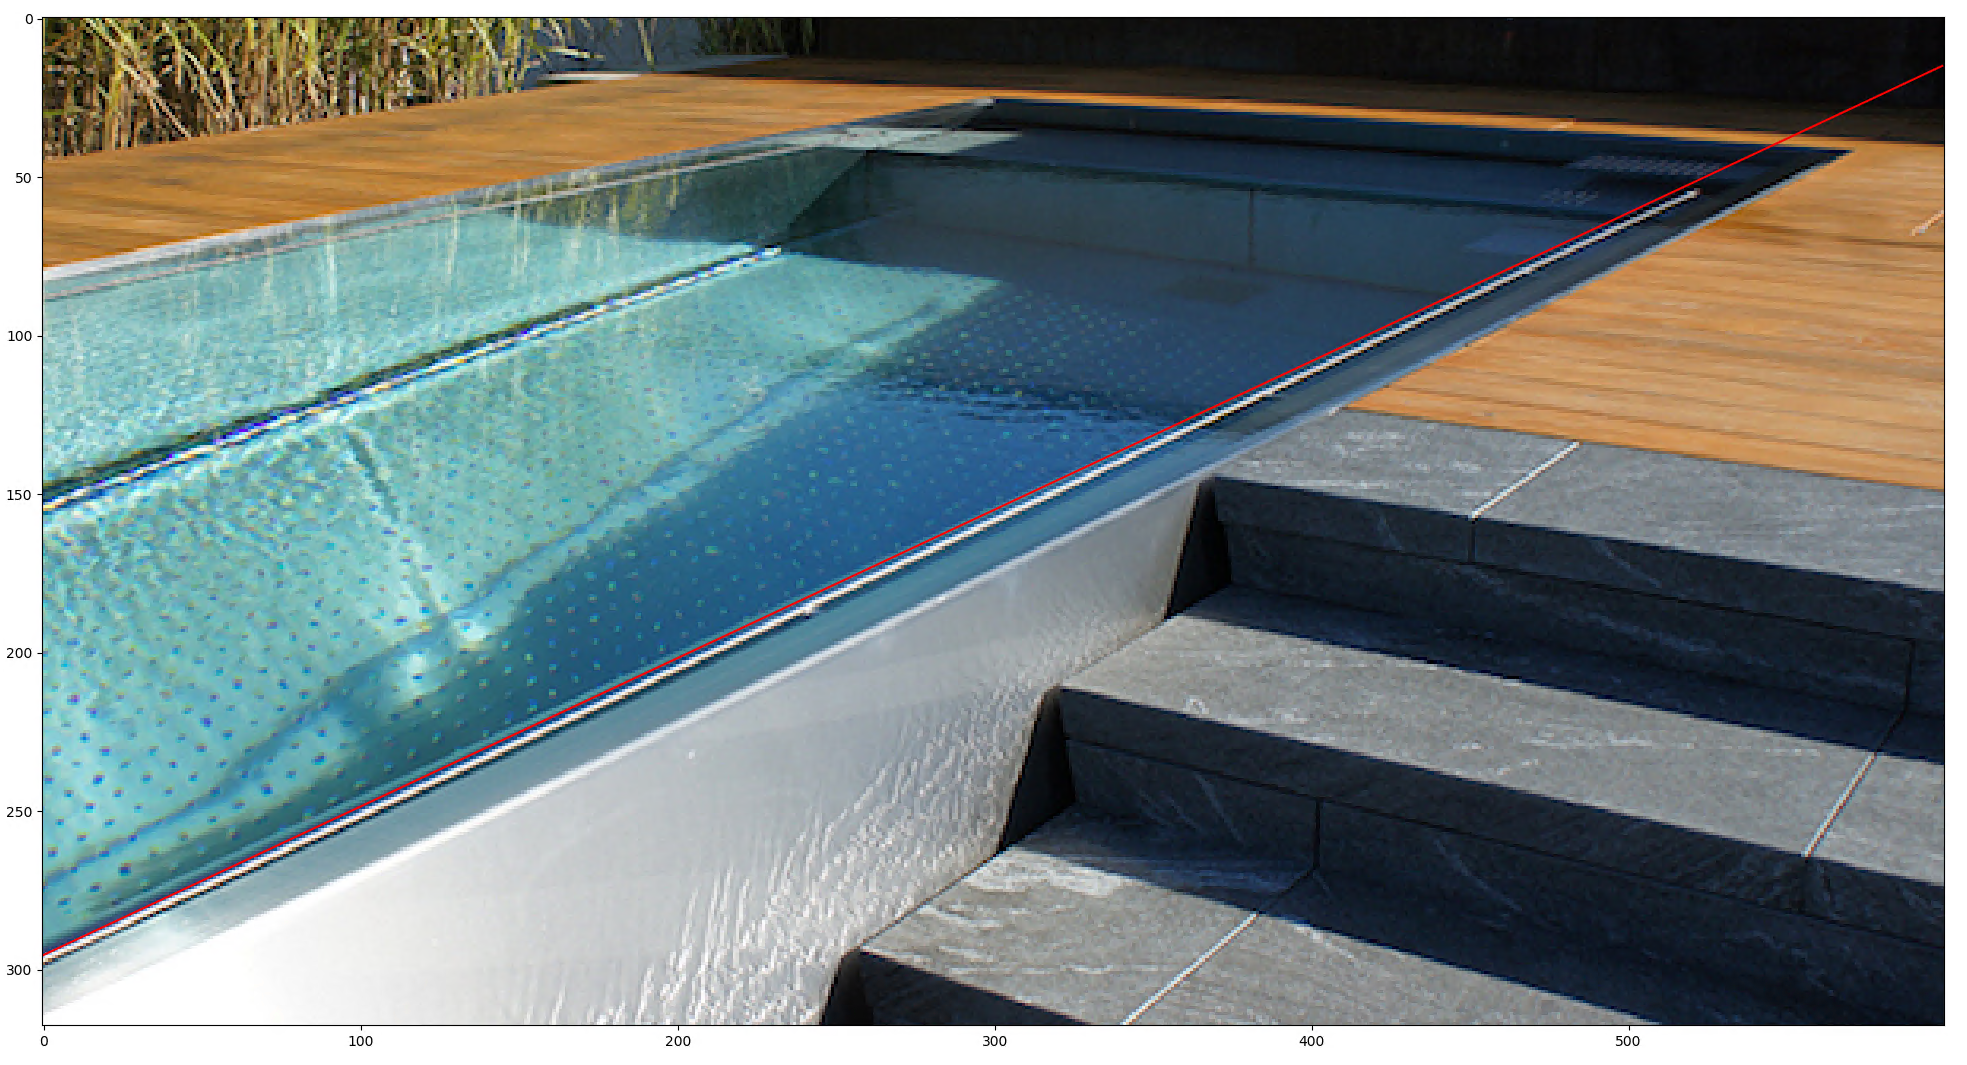
\includegraphics[width=0.95\linewidth]{pics/pool}
    \caption{result}
   \end{subfigure}
  \caption{Calculations of pool.jpg}
\end{figure}

\pagebreak

\begin{figure}[!htb]
  \centering
  \begin{subfigure}{.5\textwidth}
    \centering
    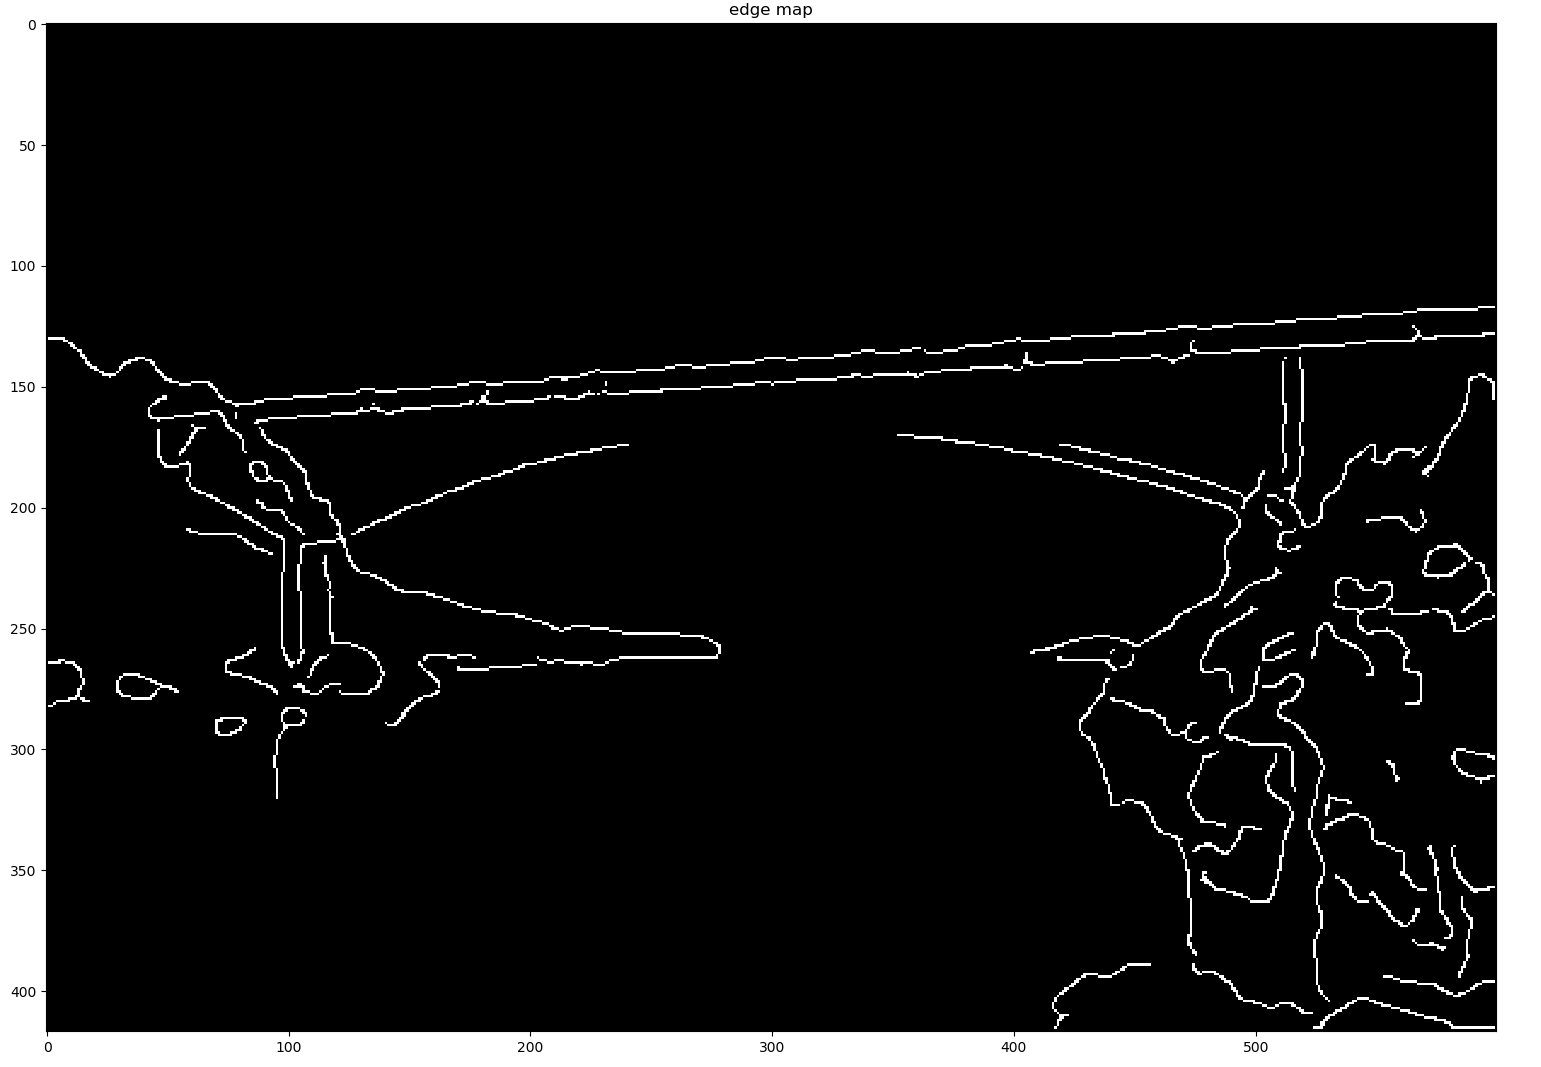
\includegraphics[width=0.95\linewidth]{pics/bridgeEdgeMap}
    \caption{edge map}
  \end{subfigure}%
  \begin{subfigure}{.5\textwidth}
    \centering
    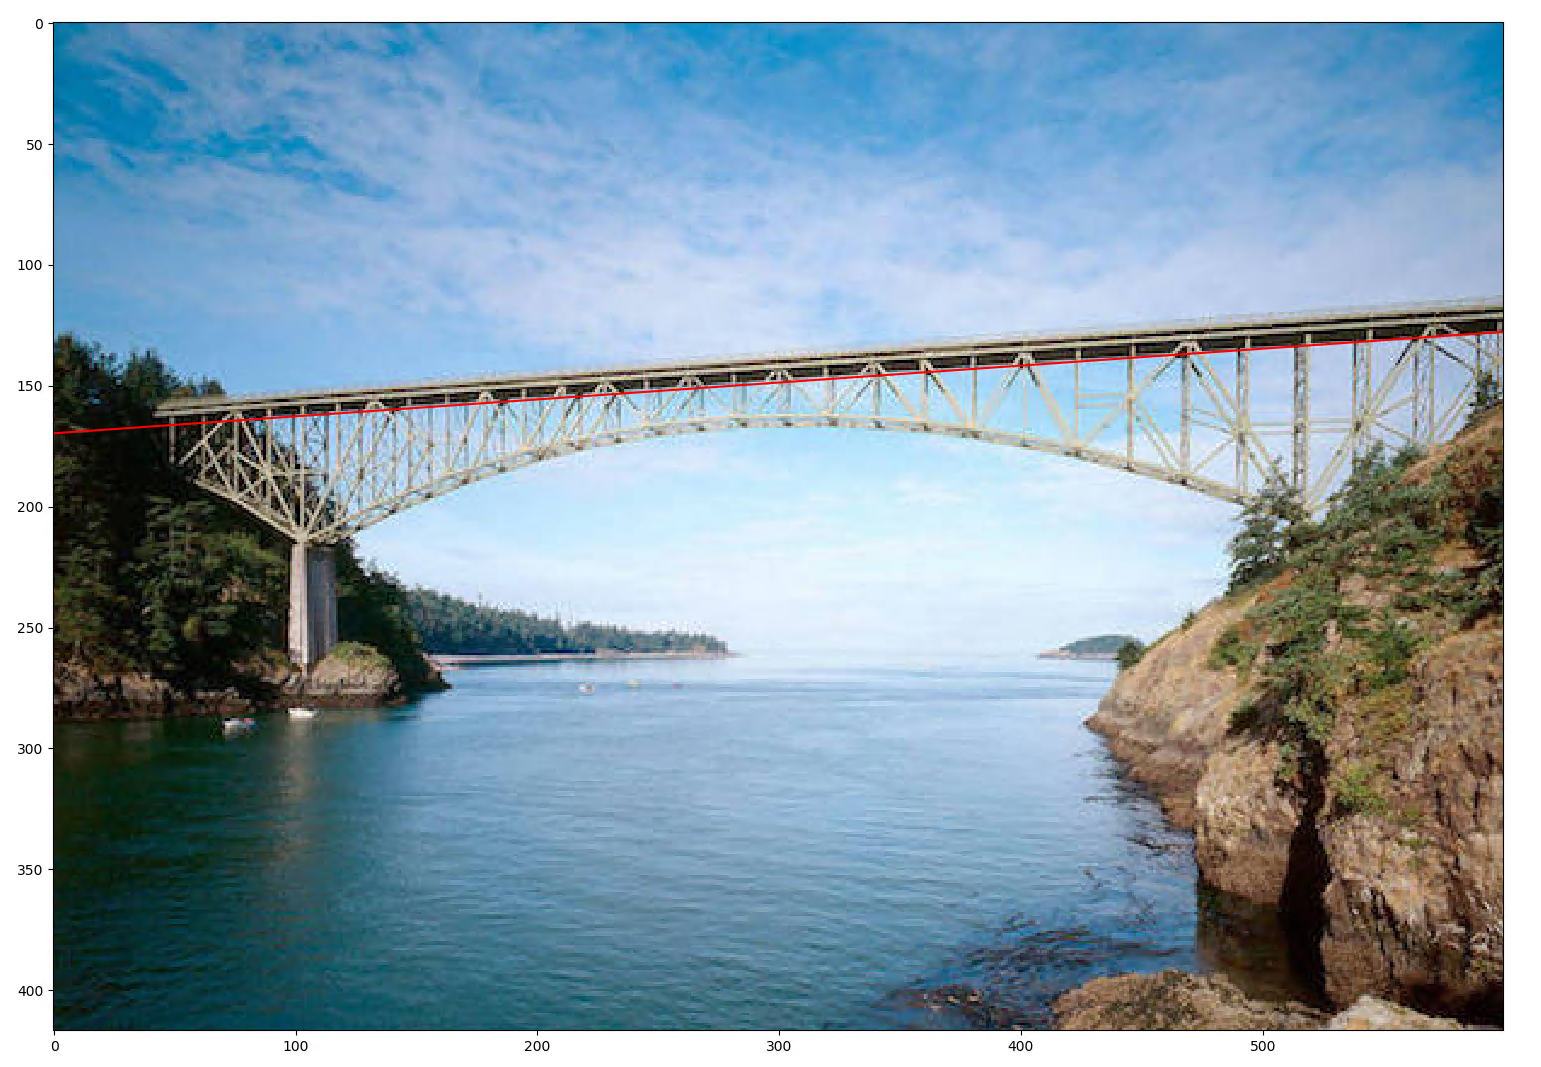
\includegraphics[width=0.95\linewidth]{pics/bridge}
    \caption{result}
   \end{subfigure}
  \caption{Calculations of bridge.jpg}
\end{figure}

\begin{figure}[!htb]
  \centering
  \begin{subfigure}{.5\textwidth}
    \centering
    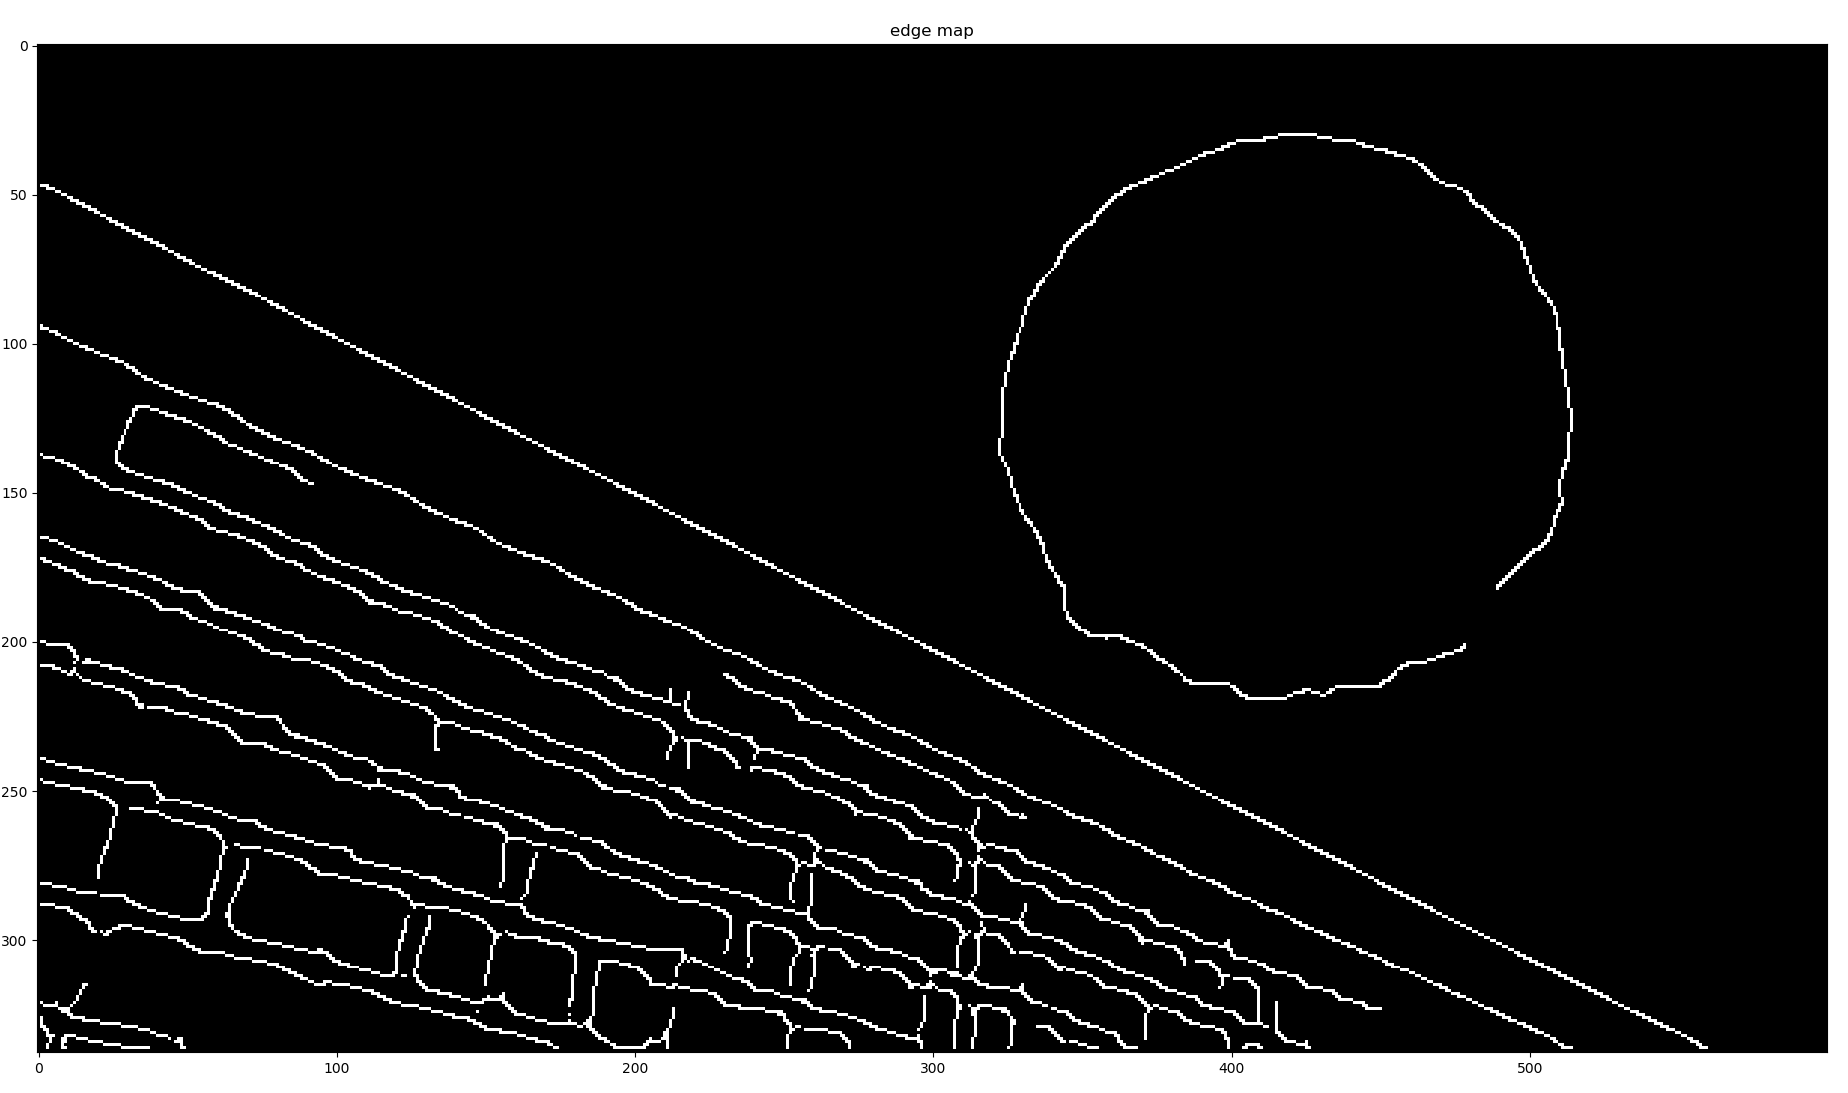
\includegraphics[width=0.95\linewidth]{pics/tennisEdgeMap}
    \caption{edge map}
  \end{subfigure}%
  \begin{subfigure}{.5\textwidth}
    \centering
    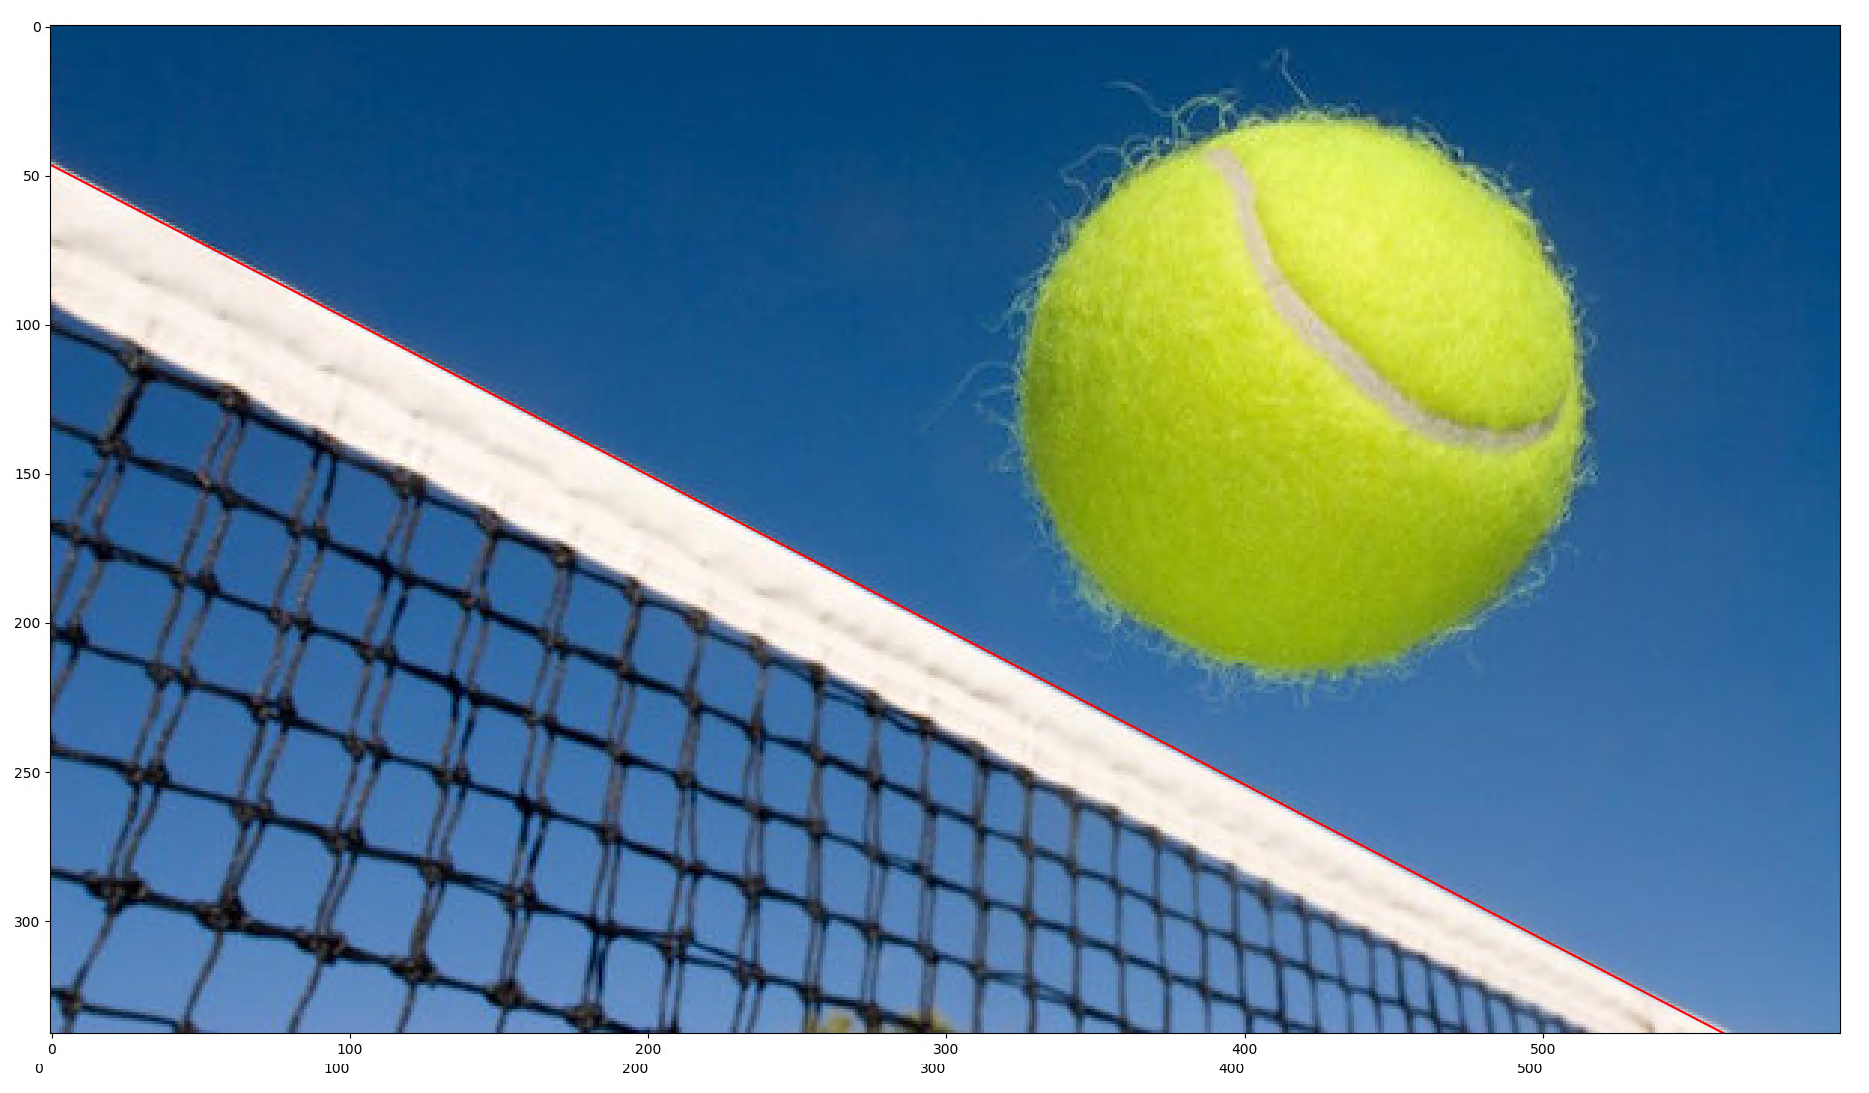
\includegraphics[width=0.95\linewidth]{pics/tennis}
    \caption{result}
   \end{subfigure}
  \caption{Calculations of tennis.jpg}
\end{figure}

The results are identical with the to be achieved goals in the assignment. Canny with sigma 1.5 was a good choice, as it returns 
well recognizable edges to be detected by the RANSAC algorithm.

\pagebreak

\section{Texture Synthesis}
\subsection{Introduction}
The algorithm writen for this assignment tries to predict how to fill the empty space in the image
based on a sample texture from the image itself. This is done by firstly analyzing every pixel at
the corner of the missing part and with the weighted sum of all the neigbourhood pixels. The neigbourhood
is given by the patch size. The SSD determines which pixel can be used to fill the missing space in the image.
\subsection{Exercises}
\subsubsection{compute\_ssd}
For all possible locations of the patch in texture\_img computes the SSD for all pixels where mask is 0.
\newline
It was difficult to achieve a satisfying performance. Different approaches were tried before finding the best result
in a single loop solution. This might seem obvious as a nested loop always requires more time, but here it was difficult
to break the code down to a single one. 
\subsubsection{copy\_patch}
This task was not as difficult as the previous one. The best results could be achieved with the image being in range 0 to 255.
\subsection{Results}
\begin{figure}[!htb]
    \centering
    %omit extension of file. pdflatex will convert to pdf automatically.
    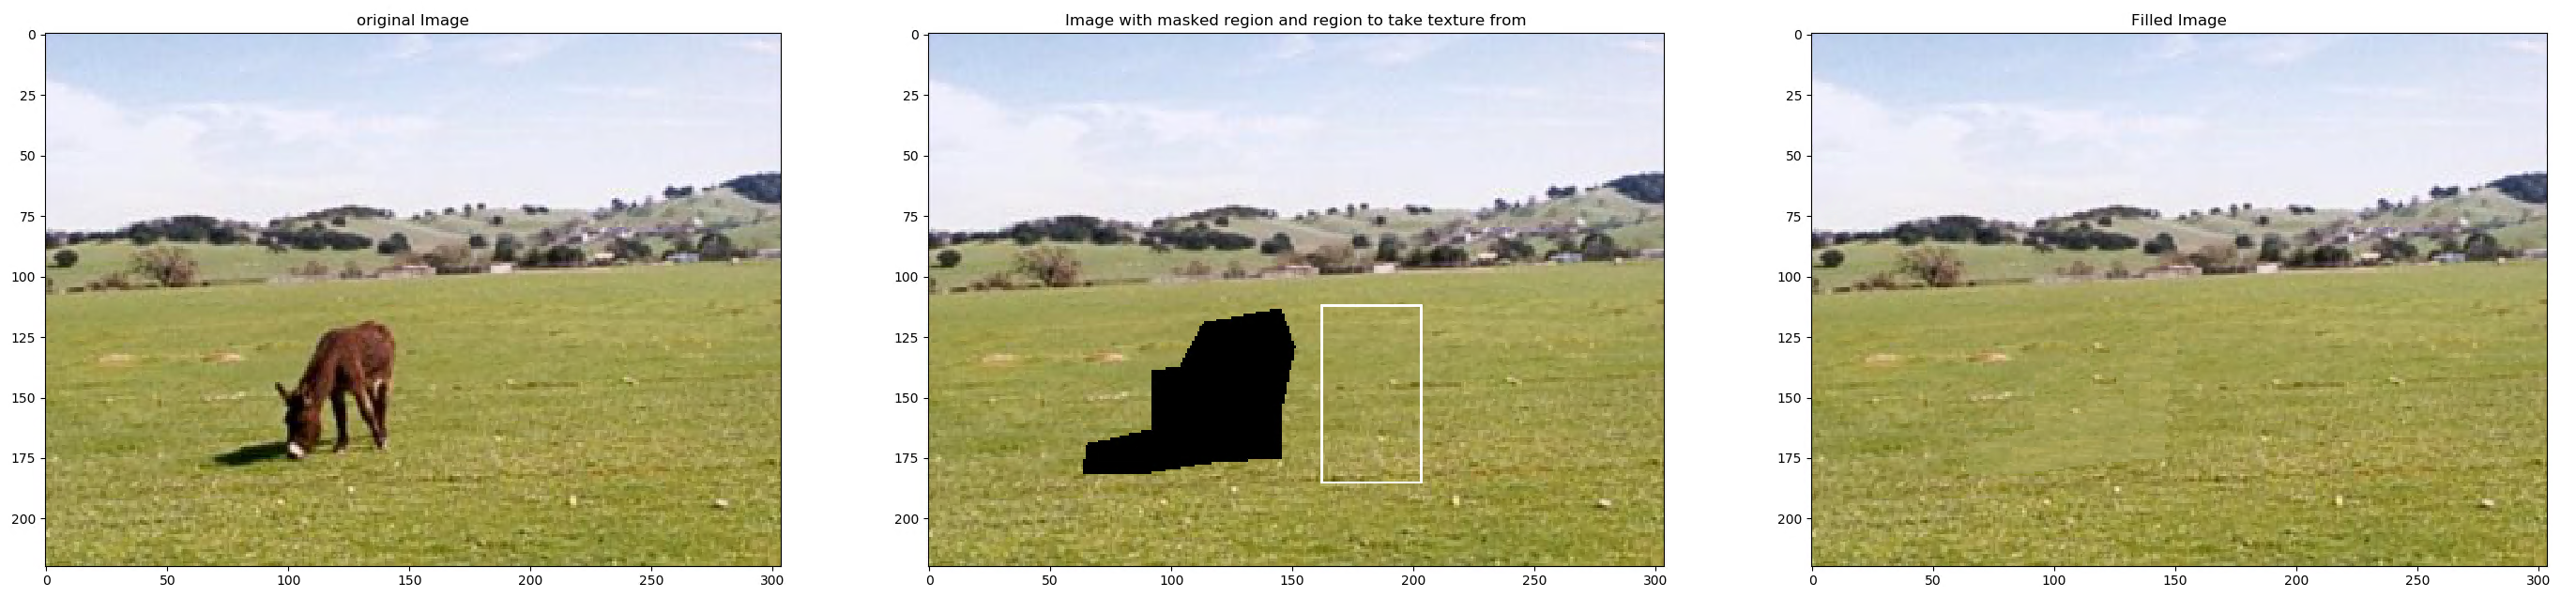
\includegraphics[width=.8\textwidth]{pics/donkey10}
    \caption{With patch of size 10}
    \end{figure}

    

    \begin{figure}[!htb]
        \centering
        %omit extension of file. pdflatex will convert to pdf automatically.
        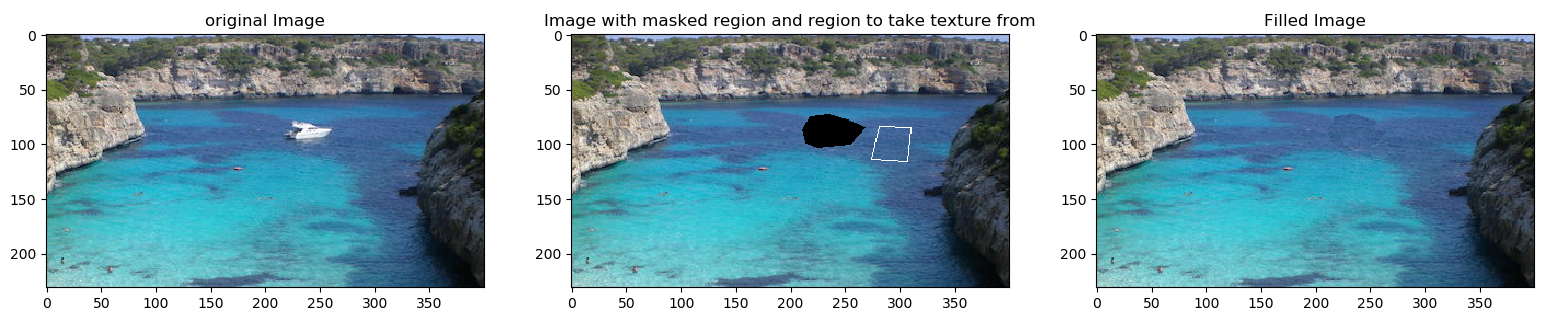
\includegraphics[width=.8\textwidth]{pics/yacht10}
        \caption{With patch of size 10}
        \end{figure}

\pagebreak

\begin{figure}[!htb]
    \centering
    %omit extension of file. pdflatex will convert to pdf automatically.
    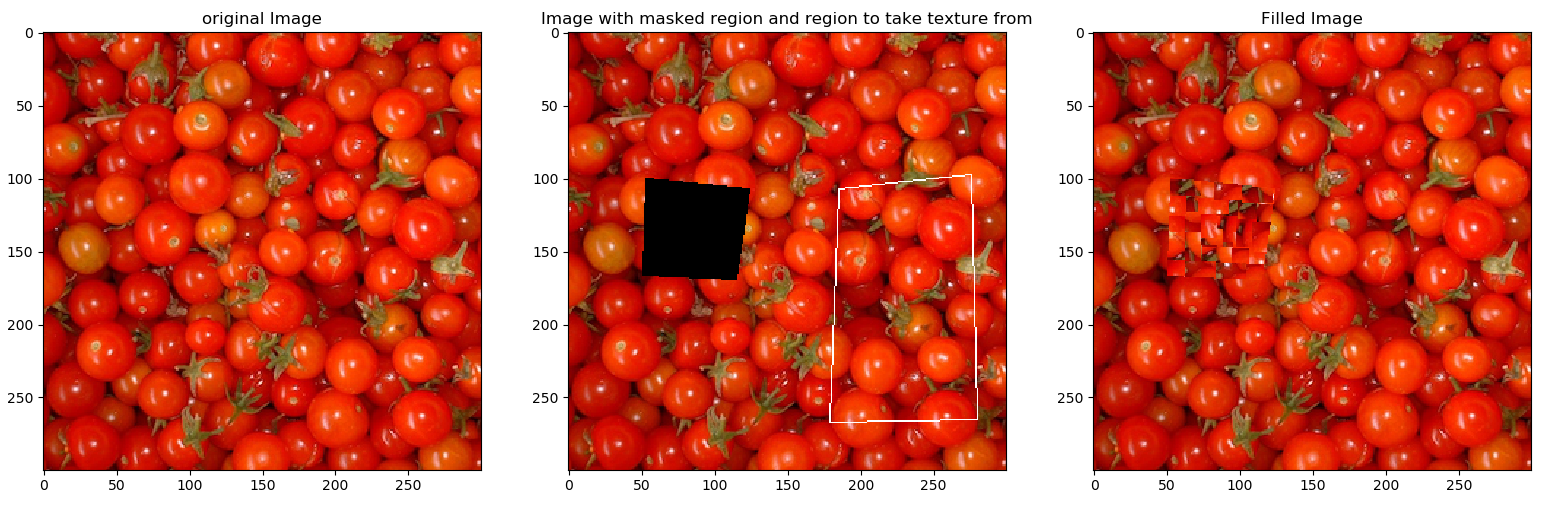
\includegraphics[width=.8\textwidth]{pics/tomato10}
    \caption{With patch of size 10}
    \end{figure}

\begin{figure}[!htb]
    \centering
    %omit extension of file. pdflatex will convert to pdf automatically.
    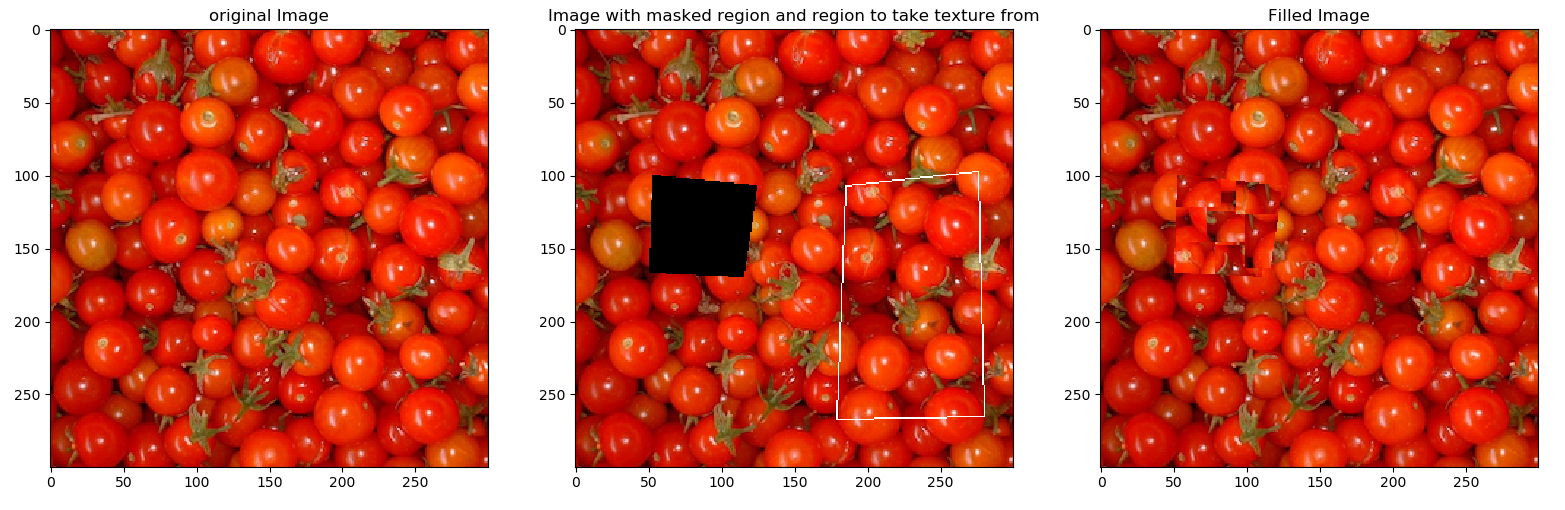
\includegraphics[width=.8\textwidth]{pics/tomato20}
    \caption{With patch of size 20}
    \end{figure}

Both for the donkey and the yacht image, a patch size of 10 yields really good resulsts.
In the tomato picture, however, one can clearly see that the patterns do not match. Trying 
a patch of size 20 for the tomato returns a slightly better result, though not satisfactory.
\newline
The results for donkey and yacht are better, because the textrue is consistent throughout 
the empty space as well as in the patch area. Therefore it doesn't really matter which part
of the patch is taken to fill.
\newline
What is different to the tomato picture is, that there is no consistent texture which makes it 
a lot harder to fill the empty space with a good result.

\section{Conclusion}
It was an interesting assignment, especially since before I haven't heard of the RANSAC algorithm or SSD.
So to not only get to know them, but also implement in a project surely was difficult though a fun thing to do.

\end{document}